
\newpage{}
\section{Observation Models}

\subsection{Landmark Tracking}
\textcolor{red}{Marie's Thesis + Michael. Model is similar to VLBI model.}

\textcolor{red}{2.1.1 In D.Dirkx for better notation.}

\textcolor{red}{Moyer, formulation for observed and computed quantities in DSN types.}
\subsection{Range Measurements/ Pseudorange}


\subsection{Doppler Measurements}

\subsubsection{Two-way Range Rate}
\begin{equation}
    \overline{\dot{\rho}}(t) = \frac{c}{2}\frac{(\tau_{2u}+\tau_{2d})-(\tau_{1u}+\tau_{2d})}{t_c} = \frac{1}{2}\frac{(\rho_{2u}+\rho_{2d})-(\rho_{1u} + \rho_{1d})}{t_c},
\end{equation}

\subsubsection{Range}

\subsubsection{One-Way Range Rate}
\begin{equation}
    \overline{\dot{\rho}} = c\frac{(\tau_2-\tau_1)}{t_c}=\frac{(\rho_2-\rho_1)}{t_c} 
\end{equation}

\subsubsection{Rational Doppler Bias}
\textcolor{red}{No real need to discuss, cut out in post processing.}
\begin{equation}
    \delta\overline{\dot{\rho}} = \frac{1}{t_c}\int_{t-t_c}^{t}d\cdot{\omega\sin{\alpha}\sin{\omega{t}}\;dt}
\end{equation}

\begin{equation}
    \Delta{\overline{\dot{\rho}}} = \frac{\lambda\omega}{2\pi}\frac{s_R+s_T/T_{1,2}}{2}
\end{equation}


\newpage{}

\section{Parameter Estimation}

\begin{itemize}
    \item Orbit of asteroid
    \item Orbit of spacecraft
    \item Rotation of asteroid (rate + principle axes)
    \item Gravitational potential of asteroid
\end{itemize}

\subsection{Orbit Determination}

\subsubsection{Weighted Least-Squares Estimation}

\begin{equation}
    H=\frac{\partial{\mathbf{h}}}{\partial{\mathbf{q}}}
\end{equation}

\begin{equation}
    \Delta{\mathbf{q}}=K(H^{T}W\Delta{\mathbf{h}})
\end{equation}

\begin{equation}
    K=(H^{T}WH)^{-1}
\end{equation}

\subsubsection{Linearization \& Normal Equations}

\subsubsection{Filtering}


 \noindent{}A CEKF consists of 3 main steps, namely: \textit{Initialisation (0)}, \textit{Prediction (1)} and \textit{Correction (2)}, where steps 1 \& 2 are iterated through $K-1$ times, where $K$ ($K\in\mathbb{Z}^+$) quantifies the number of Epochs.
 
 \begin{itemize}
     \item \textbf{Step (0) Initialisation}: The \textit{a posteriori} estimate of the initial state ($\hat{x}_0^+$) is determined according to the expectation of the true value $x_0$. The initial state error co-variance matrix is calculated according to the expectation of the co-variance between $\hat{x}_0^+$ and $x_0$. Within the context of satellite tracking, a predefined $\hat{x}_0^+$ will be used throughout the CEKF analysis to analyse the performance as a result of the selection of hyper-parameters: $\bm{Q}_{k-1}$ and $\bm{R}_k$.
     \item \textbf{Step (1) Prediction}: Project the state and its co-variance matrix at $k-1$ one step forward in order to obtain the \textit{a priori} estimates at $k$ according to the system dynamics. $\bm{Q}_{k-1}$ is implemented, then this contributes to the \textit{a priori} estimate of $P_k^{}$.
    \item \textbf{Step (2) Correction}: The measurements at $k$ are then compared with the predicted state according to system dynamics (\textit{a priori} estimate) providing the \textit{measurement innovation} ($\Delta{\rho}_k$). \textit{innovation co-variance} ($S_k$) and $H_k$ are then calculated and used to obtain the \textit{Kalman gain} ($\overline{K}_k$). Finally the \textit{a posteriori} estimate of the state ($\hat{x}_k^+$) and co-variance ($P_k^+$) are determined. $k$ is incremented by a step forward and the process from step 1 is repeated for all Epochs.
 \end{itemize}

\begin{figure}[htp]
    \centering
    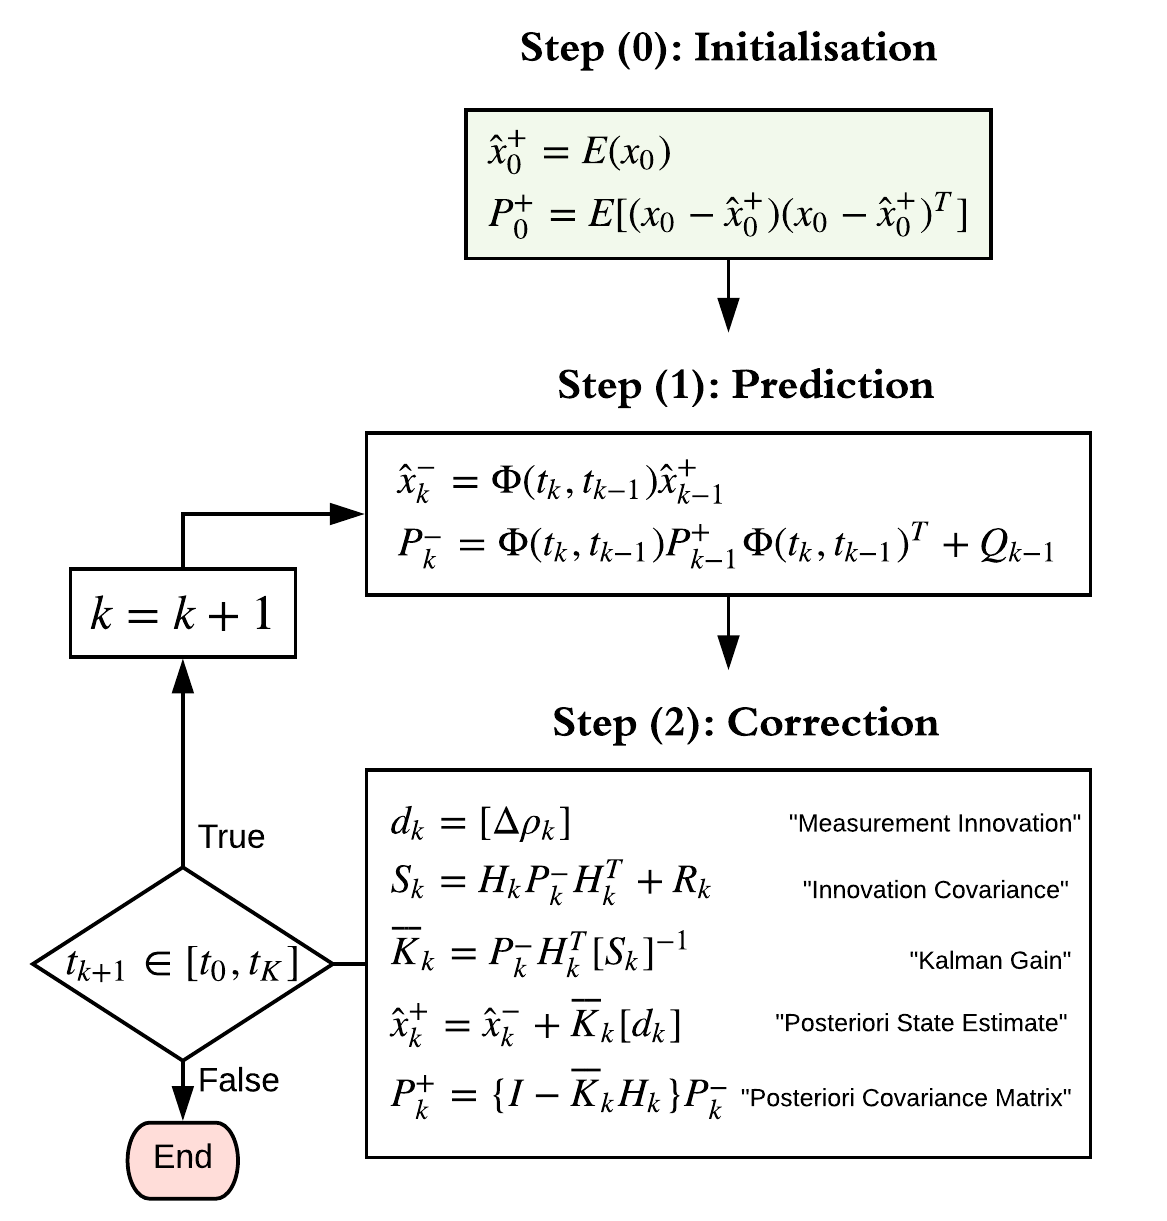
\includegraphics[width=0.55\linewidth]{graphics/CEKF.png}
    \caption{CEKF flow diagram for process of tracking and data prediction including all equations \cite{3}.}
    \label{fig:CEKF}
\end{figure}


\begin{figure}[htp]
    \centering
    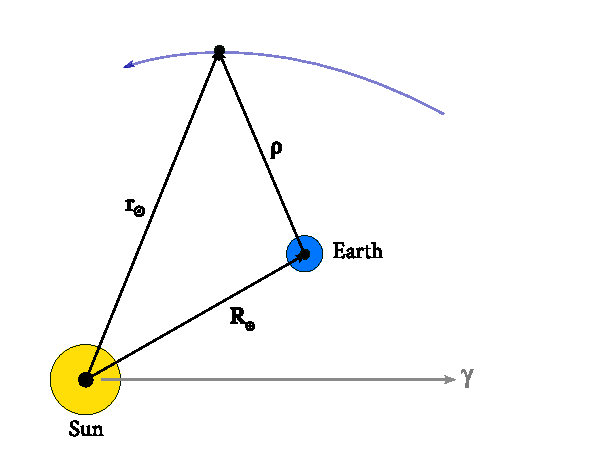
\includegraphics[width=0.5\linewidth]{graphics/pod-1.pdf}
    \caption{Orbit determination of asteroid using range observations from Earth ($\rho$).}
    \label{fig:my_label}
\end{figure}

\begin{equation}
    \rho = ||\mathbf{r}_\Sun - \mathbf{R}_\Earth||
\end{equation}


\begin{equation}
    \rho = ||\mathbf{r}_\Sun - \mathbf{R}_\Earth||
\end{equation}

\begin{itemize}
    \item \textbf{Orbit Determination}
    \item 
\end{itemize}

\subsection{Rotational State}

\subsection{Gravitational Potential}

\subsection{Shape}

\begin{itemize}
    \item \textbf{Rotation Model}: 
\end{itemize}